\documentclass[../main.tex]{subfiles}
\graphicspath{{\subfix{../images/}}}
\begin{document}
\textbf{ Quelques Images du Thème}
    \begin{figure}[bh]
        \centering
                \caption{In His LAB}
        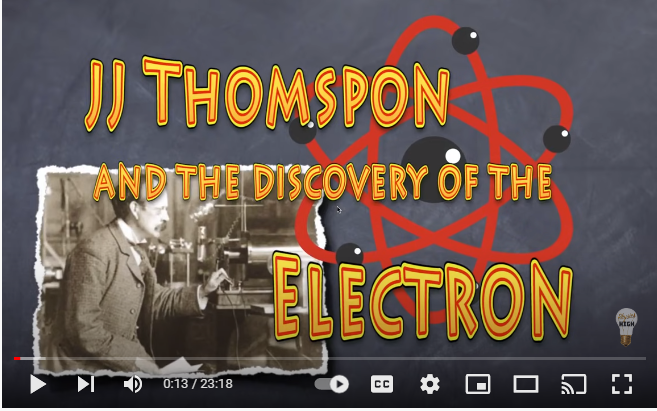
\includegraphics[width=6cm]{00.JJ-THOMSON-EXp} 
         \caption{JJ Thomson and the discovery of the electron}
        \label{fig:img1}
            \end{figure}
    19.Transcript-JJ THO-EXP
    
    
\section{JJ Thomson and the discovery of the electron}
\href{https://www.youtube.com/watch?v=GR9A7Hd4mxQ}{PhysicsHigh ; \ \textbf{JJ Thomson and the discovery of the electron}}\\

\subsection{Retranscription}
\begin{enumerate}
   \item \hspace*{.5cm} \emph{ français }
   \item Welcome to high physically.
   \item Today I'm going to make a video on JJ. Thomson on his discovery of the electron
    
    \begin{enumerate}
   \item First level item
   \item First level item
   \begin{enumerate}
     \item Second level item
     \item Second level item
     \begin{enumerate}
       \item Third level item
       \item Third level item
       \begin{enumerate}
         \item Fourth level item
         \item Fourth level item
       \end{enumerate}
     \end{enumerate}
   \end{enumerate}
 \end{enumerate}
     \end{enumerate}
    
\end{document}